\chapter{Single-Cell and Spatial Multiomics}
\label{ch:multiomics}

\begin{sourcebox}
Joint transcript and surface-protein measurement and weighted multimodal analysis are anchored by CITE-seq and Seurat method papers \cite{stoeckius2017,hao2021}. Co-measurement reduces, but does not eliminate, measurement error or the need for causal validation of inferred regulatory links.
\end{sourcebox}

\begin{keyconcept}
Multiomics refers to the simultaneous measurement of two or more molecular modalities---such as the transcriptome, epigenome, proteome, or genome---from the same individual cell or spatial location. By capturing multiple layers of biological information together, multiomics technologies resolve cellular states with far greater precision than any single assay alone, enabling the reconstruction of gene regulatory networks, lineage hierarchies, and tissue architectures that would otherwise remain hidden.
\end{keyconcept}

\section{The Promise of Multiomics}
\label{sec:multiomics:promise}

Every cell in a multicellular organism contains the same genome, yet cells adopt spectacularly different identities. This diversity arises from the interplay of multiple regulatory layers: which genes are transcribed (transcriptome), which genomic regions are accessible (epigenome), which proteins are displayed on the cell surface (proteome), and how these layers interact in space and time. Traditional single-cell technologies measure only one of these layers at a time. When different modalities are profiled in separate experiments on separate cells, computational integration is required---and the results are inherently inferential rather than directly observed.

Multiomics technologies eliminate this inference gap by measuring two, three, or even more modalities from the \textit{same individual cell}. This direct co-measurement has several transformative advantages:

\begin{itemize}[itemsep=3pt]
  \item \textbf{Direct linkage:} One can directly correlate, for example, the accessibility of a chromatin peak with the expression of its target gene in the same cell, rather than relying on statistical association across different cell populations.
  \item \textbf{Regulatory network inference:} By observing which transcription factor binding sites are open and which genes are expressed in the same cell, one can reconstruct gene regulatory networks with far greater confidence.
  \item \textbf{Cell-type resolution:} Surface protein markers (measured by CITE-seq) can provide ``ground truth'' cell-type labels that are more robust than transcriptome-only clustering, particularly for closely related cell states.
  \item \textbf{Lineage and trajectory analysis:} Joint measurement of genetic barcodes (or somatic mutations) alongside transcriptomic state enables simultaneous tracking of cell identity and cell history.
\end{itemize}

\begin{warningbox}
Multiomics experiments are substantially more expensive per cell than single-modality assays, and the data generated are more complex to analyse. In many cases, a well-designed single-modality experiment with appropriate computational integration will answer the biological question more cost-effectively. Multiomics is most valuable when direct co-measurement is scientifically essential---for example, linking specific regulatory elements to target genes or resolving ambiguous cell states.
\end{warningbox}


\section{Joint RNA + Chromatin Accessibility}
\label{sec:multiomics:rna-atac}

The joint profiling of gene expression and chromatin accessibility within the same cell represents one of the most mature and widely adopted multiomics modalities. By measuring both the transcriptome (what is being expressed) and the accessible chromatin landscape (what \textit{could} be expressed), these assays provide a direct window into the regulatory logic of individual cells.

\subsection{10x Genomics Multiome (ATAC + GEX)}
\label{subsec:multiomics:10x-multiome}

The 10x Genomics Multiome kit is currently the most widely used commercial platform for joint single-nucleus ATAC-seq and gene expression profiling. The assay works on \textit{nuclei} rather than whole cells, which is important for understanding its characteristics.

\begin{protocolbox}[title={10x Multiome ATAC + GEX Protocol Overview}]
\begin{enumerate}[itemsep=2pt]
  \item \textbf{Nuclear isolation:} Cells are lysed and nuclei are isolated. This step is critical---overly harsh lysis destroys chromatin structure, while insufficient lysis leaves cytoplasmic RNA behind.
  \item \textbf{Transposition:} Nuclei are incubated with Tn5 transposase loaded with sequencing adapters. Tn5 inserts adapters preferentially into accessible (open) chromatin regions.
  \item \textbf{GEM generation:} Transposed nuclei are loaded onto the Chromium controller, where each nucleus is captured in a gel bead-in-emulsion (GEM) droplet with a uniquely barcoded gel bead.
  \item \textbf{Barcoding:} Within each GEM, the nuclear RNA is reverse-transcribed and barcoded, while the transposed ATAC fragments are simultaneously barcoded with the same cell barcode.
  \item \textbf{Library construction:} After breaking the emulsion, ATAC and GEX libraries are separated and independently amplified for sequencing.
  \item \textbf{Sequencing:} Both libraries are sequenced on Illumina instruments. The shared cell barcode links ATAC and GEX data from the same nucleus.
\end{enumerate}
\end{protocolbox}

Typical throughput is 500--10,000 nuclei per experiment, with the recommended sequencing depth of approximately 25,000 read pairs per nucleus for ATAC and 20,000 read pairs per nucleus for GEX.

\subsection{SHARE-seq, SNARE-seq, and Paired-seq}
\label{subsec:multiomics:share-snare-paired}

Before the 10x Multiome became commercially available, several academic methods established the feasibility of joint RNA + ATAC profiling:

\begin{description}[style=nextline, itemsep=3pt]
  \item[SHARE-seq (Simultaneous High-throughput ATAC and RNA Expression with Sequencing)] Developed by the Bhatt and Bhatt laboratories, SHARE-seq uses a split-pool combinatorial barcoding strategy rather than droplet-based encapsulation. This allows profiling of many more cells (up to hundreds of thousands) without requiring a microfluidics instrument. SHARE-seq was notably used to discover ``domain of regulatory chromatin'' (DORC) scores, linking accessible chromatin regions to gene expression.

  \item[SNARE-seq (Single-Nucleus Chromatin Accessibility and mRNA Expression Sequencing)] An earlier droplet-based method that captures both modalities from single nuclei. SNARE-seq2 improved throughput significantly using a modified barcoding strategy.

  \item[Paired-seq] Another combinatorial indexing approach that scales to hundreds of thousands of cells, with the advantage of being instrument-free (no microfluidics device required).
\end{description}

\subsection{Analysis: Linking Peaks to Genes}
\label{subsec:multiomics:peak-gene-linking}

The central analytical goal of joint RNA + ATAC data is to link cis-regulatory elements (ATAC peaks) to their target genes. Several strategies are used:

\begin{enumerate}[itemsep=3pt]
  \item \textbf{Correlation-based linking:} For each peak--gene pair within a defined genomic window (e.g., 250\kilobase{} of the gene's TSS), compute the correlation between peak accessibility and gene expression across cells. Statistically significant positive correlations suggest a regulatory relationship.
  \item \textbf{Transcription factor motif enrichment:} Identify transcription factor (TF) binding motifs enriched in linked peaks, then correlate TF expression with both peak accessibility and target gene expression to build a regulatory circuit.
  \item \textbf{Gene regulatory network (GRN) inference:} Tools such as \software{SCENIC+} extend the SCENIC framework to jointly model TF expression, TF motif accessibility, and target gene expression, producing comprehensive GRN models.
\end{enumerate}

\begin{keyconcept}[title={Vertical vs.\ Diagonal Integration}]
When RNA and ATAC data come from the \textit{same cells} (as in 10x Multiome), this is called \textbf{vertical integration}---one simply links the modalities via the shared cell barcode. When the two modalities are measured in \textit{different cells} (e.g., separate scRNA-seq and scATAC-seq experiments), computational \textbf{diagonal integration} is needed, using methods such as those in Seurat v5, \software{ArchR}, or \software{MultiVI}. Vertical integration is always preferable when feasible because it avoids the assumptions inherent in cross-modality alignment.
\end{keyconcept}

\subsection{Peak-to-Gene Correlation Framework}
\label{subsec:multiomics:peak-gene-correlation}

The correlation-based linking of ATAC peaks to target genes is the foundational analysis for joint RNA + chromatin data. The statistical framework operates as follows. For a given gene $g$ and a candidate cis-regulatory peak $p$ located within a genomic distance window $d_{\max}$ (typically 250--500\kilobase{}) of the gene's transcription start site, one computes the correlation between chromatin accessibility and gene expression across all cells:
\begin{equation}
  r_{pg} = \text{cor}\bigl(\mathbf{a}_p,\; \mathbf{x}_g\bigr),
  \label{eq:multiomics:peak-gene-corr}
\end{equation}
where $\mathbf{a}_p = (a_{p1}, a_{p2}, \ldots, a_{pN})$ is the vector of accessibility values for peak $p$ across $N$ cells, and $\mathbf{x}_g = (x_{g1}, x_{g2}, \ldots, x_{gN})$ is the corresponding expression vector for gene $g$. Either Pearson or Spearman correlation may be used; Spearman is more robust to the zero-inflated nature of single-cell data.

\begin{keyconcept}[title={Significance Testing by Permutation}]
Because the large number of peak--gene pairs tested creates a severe multiple testing burden, permutation-based significance is preferred over parametric $p$-values. For each peak--gene pair, the gene expression vector is permuted $B$ times (typically $B = 1{,}000$--$10{,}000$), and the correlation is recomputed for each permutation. The empirical $p$-value is:
\begin{equation}
  p_{\text{perm}} = \frac{1 + \sum_{b=1}^{B} \mathbb{1}\bigl(|r^{(b)}_{pg}| \geq |r_{pg}|\bigr)}{1 + B},
  \label{eq:multiomics:perm-pvalue}
\end{equation}
where $r^{(b)}_{pg}$ is the correlation from the $b$-th permutation. False discovery rate (FDR) correction (Benjamini--Hochberg) is applied across all tested pairs. Only peak--gene links with positive correlation and FDR $< 0.05$ are typically retained, as enhancers are expected to activate (not repress) their target genes.
\end{keyconcept}

The resulting set of significant peak--gene links provides a map of putative enhancer--gene regulatory relationships. A useful aggregate metric is the \textbf{DORC score} (Domain of Regulatory Chromatin), introduced with SHARE-seq. For each gene, the DORC score sums the accessibility of all significantly linked peaks:
\begin{equation}
  \text{DORC}_g(i) = \sum_{p \in \mathcal{L}(g)} a_{pi},
  \label{eq:multiomics:dorc}
\end{equation}
where $\mathcal{L}(g)$ is the set of peaks significantly linked to gene $g$ and $a_{pi}$ is the accessibility of peak $p$ in cell $i$. Genes with high DORC scores are regulated by large cis-regulatory domains encompassing many accessible elements; these tend to be key cell-identity genes such as master transcription factors and lineage-defining markers. The DORC score provides a chromatin-derived proxy for gene regulatory potential that complements expression-based measures.

These links can be further validated by:
\begin{itemize}[itemsep=2pt]
  \item Overlap with known enhancer databases (e.g., ENCODE cCREs, VISTA enhancer browser).
  \item Enrichment for transcription factor binding motifs consistent with the target gene's regulatory logic.
  \item Consistency with Hi-C or promoter-capture Hi-C contact data, confirming physical proximity between the peak and the gene's promoter.
  \item Perturbation experiments (e.g., CRISPRi targeting of individual peaks) to confirm functional regulatory activity.
\end{itemize}

\begin{warningbox}
Correlation-based peak--gene linking has important caveats. First, the distance window $d_{\max}$ is arbitrary; some enhancers act over distances exceeding 1\megabase{}, while using large windows increases false positives. Second, the correlations are computed across cell types, so they primarily capture regulatory relationships that vary across cell identities rather than within a cell type. Third, negative correlations (suggesting repressive elements such as silencers) are typically discarded but may represent genuine biology. Fourth, the sparsity of single-cell ATAC data (most peaks are detected in only a small fraction of cells) limits statistical power, requiring large cell numbers ($>$5{,}000) for robust link detection.
\end{warningbox}

\subsection{Tools for Joint RNA + ATAC Analysis}
\label{subsec:multiomics:rna-atac-tools}

\begin{description}[style=nextline, itemsep=3pt]
  \item[\software{ArchR}] A comprehensive R package for single-cell ATAC-seq analysis that natively supports multiome data. Provides peak calling, motif enrichment, peak-to-gene linking, trajectory analysis, and integration with scRNA-seq. Highly memory-efficient through the use of Arrow files.

  \item[\software{Signac}] An extension of the Seurat framework for chromatin data analysis. Provides functions for quality control, dimensionality reduction, motif analysis, and integration with gene expression data from the same or different cells.

  \item[\software{MOFA+} (Multi-Omics Factor Analysis)] A Bayesian factor analysis method that identifies shared and modality-specific sources of variation across multiple data types. Particularly useful for exploratory analysis of multiomics datasets.

  \item[\software{MultiVI}] Part of the \software{scvi-tools} suite, MultiVI is a deep generative model that can jointly analyse RNA and ATAC data, handling both paired (multiome) and unpaired (separate experiments) data within a unified framework.
\end{description}

\subsection{Variational Autoencoders for Multiomics: scVI, MultiVI, and the ELBO}
\label{subsec:multiomics:vae-elbo}

Several of the most effective tools for single-cell and multiomics analysis---\software{scVI}, \software{TotalVI}, \software{MultiVI}, and \software{Cobolt}---are built on the \textbf{variational autoencoder} (VAE) framework. Understanding the underlying mathematics is essential for interpreting their outputs and choosing appropriate hyperparameters.

A VAE consists of two neural networks:
\begin{enumerate}[itemsep=2pt]
  \item An \textbf{encoder} (inference network) $q_\phi(\mathbf{z} | \mathbf{x})$ that maps the observed data $\mathbf{x}$ (e.g., a cell's gene expression vector) to a distribution over a low-dimensional latent space $\mathbf{z}$.
  \item A \textbf{decoder} (generative network) $p_\theta(\mathbf{x} | \mathbf{z})$ that reconstructs the observed data from a sample in the latent space.
\end{enumerate}

The model is trained by maximizing the \textbf{Evidence Lower BOund (ELBO)} on the log-marginal likelihood of the data:
\begin{equation}
  \text{ELBO}(\theta, \phi; \mathbf{x}) = \underbrace{\mathbb{E}_{q_\phi(\mathbf{z}|\mathbf{x})}\bigl[\log p_\theta(\mathbf{x} | \mathbf{z})\bigr]}_{\text{Reconstruction term}} - \underbrace{\text{KL}\bigl(q_\phi(\mathbf{z}|\mathbf{x}) \;\|\; p(\mathbf{z})\bigr)}_{\text{Regularization term}},
  \label{eq:multiomics:elbo}
\end{equation}
where $p(\mathbf{z})$ is the prior distribution over the latent space (typically a standard normal $\mathcal{N}(\mathbf{0}, \mathbf{I})$). The reconstruction term encourages the model to faithfully reproduce the input data, while the KL divergence regularizes the latent space to remain close to the prior, preventing overfitting and ensuring a smooth, interpretable latent representation.

\begin{keyconcept}[title={scVI: Modelling Count Data with ZINB Likelihood}]
\software{scVI} (single-cell Variational Inference) tailors the VAE framework to the specific statistical properties of scRNA-seq data. Rather than using a Gaussian reconstruction loss, scVI models gene expression counts with a \textbf{zero-inflated negative binomial} (ZINB) distribution:
\begin{equation}
  p(x_g | \mathbf{z}, s) = \pi_g \,\delta_0(x_g) + (1 - \pi_g)\,\text{NB}(x_g;\, \mu_g,\, \theta_g),
  \label{eq:multiomics:zinb}
\end{equation}
where $x_g$ is the observed count for gene $g$, $\pi_g$ is the zero-inflation probability (modelling technical dropouts), $\mu_g$ is the mean expression (a function of $\mathbf{z}$ and the library size $s$), and $\theta_g$ is the gene-specific dispersion parameter. The decoder network outputs $\pi_g$, $\mu_g$, and $\theta_g$ for each gene. Batch effects are handled by conditioning the decoder on a batch indicator variable, enabling integrated analysis across experiments without explicit batch correction.
\end{keyconcept}

\software{MultiVI} extends the scVI framework to jointly model RNA and ATAC data. The key innovations are:
\begin{itemize}[itemsep=2pt]
  \item A shared latent space $\mathbf{z}$ that captures biological variation common to both modalities.
  \item Modality-specific decoder heads: a ZINB decoder for RNA counts and a Bernoulli decoder for binarized ATAC peaks.
  \item The ability to handle \textbf{unpaired data}: cells with only RNA, cells with only ATAC, and cells with both modalities are all incorporated into a single model. Missing modalities are treated as latent variables and imputed by the decoder.
  \item The ELBO for MultiVI sums the reconstruction terms for both modalities:
  \begin{equation}
    \text{ELBO}_{\text{MultiVI}} = \mathbb{E}_{q(\mathbf{z}|\mathbf{x}_{\text{RNA}}, \mathbf{x}_{\text{ATAC}})}\bigl[\log p(\mathbf{x}_{\text{RNA}} | \mathbf{z}) + \log p(\mathbf{x}_{\text{ATAC}} | \mathbf{z})\bigr] - \text{KL}\bigl(q(\mathbf{z}|\mathbf{x}) \| p(\mathbf{z})\bigr).
    \label{eq:multiomics:multivi-elbo}
  \end{equation}
\end{itemize}

\begin{tipbox}[title={Practical Considerations for VAE-Based Models}]
When using scVI or MultiVI, several hyperparameters require attention:
\begin{itemize}[itemsep=2pt]
  \item \textbf{Latent dimension:} Typically 10--30. Larger values capture more variation but risk overfitting with small datasets.
  \item \textbf{Number of hidden layers and neurons:} Default architectures (1--2 hidden layers, 128--256 neurons) work well for most datasets up to $\sim$500{,}000 cells.
  \item \textbf{KL annealing:} Gradually increasing the weight of the KL term during training (``warm-up'') prevents posterior collapse, where the encoder ignores the data and collapses to the prior.
  \item \textbf{Training epochs:} Monitor the ELBO on a held-out validation set; training for 200--400 epochs is typical. Early stopping prevents overfitting.
\end{itemize}
\end{tipbox}

\subsection{Gene Regulatory Network Inference with SCENIC+}
\label{subsec:multiomics:grn-inference}

Gene regulatory network (GRN) inference from multiomics data aims to reconstruct the regulatory logic connecting transcription factors (TFs), their binding sites in accessible chromatin, and their target genes. The \software{SCENIC+} pipeline is the most comprehensive approach for joint RNA + ATAC data and operates in three stages:

\begin{enumerate}[itemsep=3pt]
  \item \textbf{TF motif enrichment in accessible regions:} For each cell cluster or cell type, \software{SCENIC+} identifies ATAC peaks enriched for known TF binding motifs using tools such as \software{cisTarget}. This produces a set of candidate TF--region associations: TF $t$ is linked to peak $p$ if the motif for $t$ is significantly enriched in $p$.

  \item \textbf{TF--target gene regression (GRNBoost2):} \software{GRNBoost2} uses gradient-boosted tree regression to model the expression of each gene as a function of TF expression levels across cells:
  \begin{equation}
    x_g = f_g\bigl(x_{t_1}, x_{t_2}, \ldots, x_{t_K}\bigr) + \epsilon_g,
    \label{eq:multiomics:grnboost2}
  \end{equation}
  where $x_g$ is the expression of target gene $g$, $x_{t_k}$ is the expression of the $k$-th transcription factor, and $f_g$ is a non-linear function learned by the ensemble of gradient-boosted trees. The importance score for each TF--gene pair is derived from the feature importance of the tree ensemble. GRNBoost2 is preferred over alternatives such as GENIE3 because of its substantially faster runtime on large single-cell datasets.

  \item \textbf{Filtering by motif support:} TF--gene links from the regression step are retained only if the TF's binding motif is found in an accessible peak linked to the target gene (from step 1). This intersection of expression-based and motif-based evidence yields high-confidence \textbf{regulons}---sets of target genes regulated by a common TF, supported by both co-expression and cis-regulatory motif evidence.
\end{enumerate}

The final output of SCENIC+ is a GRN consisting of TFs, their regulons, and the associated cis-regulatory regions, providing a multi-layered view of gene regulation in each cell type. For each TF $t$ and its regulon $\mathcal{R}_t$, SCENIC+ computes a \textbf{regulon activity score} (RAS) for each cell $i$:
\begin{equation}
  \text{RAS}_t(i) = \frac{1}{|\mathcal{R}_t|} \sum_{g \in \mathcal{R}_t} \tilde{x}_{gi},
  \label{eq:multiomics:ras}
\end{equation}
where $\tilde{x}_{gi}$ is the normalized, scaled expression of target gene $g$ in cell $i$, and $|\mathcal{R}_t|$ is the size of the regulon. More sophisticated scoring methods, such as the AUCell algorithm, rank genes by expression within each cell and compute the area under the recovery curve for regulon genes, providing a score that is robust to differences in sequencing depth and drop-out rates. The regulon activity matrix (TFs $\times$ cells) can be used for clustering, trajectory analysis, and identification of master regulators for each cell state.

\begin{table}[htbp]
\centering
\caption[Comparison of GRN inference methods for single-cell multiomics.]{Comparison of gene regulatory network inference methods applicable to single-cell multiomics data.}
\label{tab:multiomics:grn-comparison}
\footnotesize
\begin{tabularx}{\textwidth}{>{\bfseries\raggedright\arraybackslash}p{1.8cm} X >{\raggedright\arraybackslash}p{2.1cm} >{\raggedright\arraybackslash}p{3.7cm}}
\toprule
\textbf{Method} & \textbf{Evidence used} & \textbf{Typical scale} & \textbf{Output} \\
\midrule
SCENIC+ & Expression regression plus accessible-region motif support & Large datasets & TF regulons with enhancer links \\
\addlinespace
CellOracle & Regression with TF-binding priors that can be derived from ATAC & Moderate & Directed GRN and in-silico perturbation \\
\addlinespace
Dictys & Joint RNA and ATAC in a context-specific dynamic model & Moderate & Dynamic, context-specific GRN \\
\addlinespace
GENIE3 & Tree-based regression of TF--gene relationships; no ATAC required & Small--moderate & TF--gene importance scores \\
\addlinespace
GRaNIE & Peak--gene correlations plus TF motif enrichment & Large datasets & TF--peak--gene triplets \\
\addlinespace
FigR & DORC-based links between TF activity and gene modules & Large datasets & TF--DORC--gene circuits \\
\bottomrule
\end{tabularx}
\end{table}

\begin{warningbox}
GRN inference from observational single-cell data is inherently correlative, not causal. Co-expression of a TF with a target gene and the presence of a TF motif in a nearby accessible peak are consistent with---but do not prove---a direct regulatory relationship. Validation through perturbation experiments (e.g., CRISPRi knockdown of the TF followed by scRNA-seq) is essential before drawing strong conclusions about regulatory causality. Additionally, GRNBoost2 and similar methods cannot distinguish direct from indirect regulation; a TF may appear to regulate a gene because both are downstream of a common upstream regulator.
\end{warningbox}


\section{Joint RNA + Protein (Surface Markers)}
\label{sec:multiomics:rna-protein}

\subsection{CITE-seq: Antibody-Derived Tags + Transcriptome}
\label{subsec:multiomics:cite-seq}

\textbf{CITE-seq} (Cellular Indexing of Transcriptomes and Epitopes by Sequencing) was developed by the Bhatt and Smibert laboratories and published in 2017. It enables simultaneous measurement of surface protein expression and the transcriptome from the same single cell.

\begin{protocolbox}[title={CITE-seq Principle}]
\begin{enumerate}[itemsep=2pt]
  \item Cells are stained with a panel of antibodies, each conjugated to a unique DNA oligonucleotide called an \textbf{antibody-derived tag (ADT)}.
  \item Stained cells are loaded onto a droplet-based single-cell platform (e.g., 10x Chromium).
  \item Within each droplet, both mRNA and ADT oligos are captured by the barcoded bead, reverse-transcribed, and barcoded with the same cell barcode.
  \item After library preparation, RNA and ADT libraries are sequenced separately, then linked by cell barcode.
  \item The number of ADT reads per cell is proportional to the abundance of the corresponding surface protein.
\end{enumerate}
\end{protocolbox}

CITE-seq has become enormously popular because it provides protein-level phenotyping (similar to flow cytometry) alongside whole-transcriptome profiling. Large antibody panels of 200+ markers are now routinely used with commercial panels from BioLegend (TotalSeq).

\subsection{REAP-seq and ASAP-seq}
\label{subsec:multiomics:reap-asap}

\textbf{REAP-seq} (RNA Expression and Protein Sequencing) is conceptually similar to CITE-seq but uses a different antibody--oligo conjugation chemistry developed by the Zhang laboratory at the New York Genome Center. \textbf{ASAP-seq} (ATAC with Select Antigen Profiling by Sequencing) extends the antibody-tagging concept to ATAC-seq, enabling joint measurement of chromatin accessibility and surface protein expression---a unique combination not achievable with CITE-seq alone.

\subsection{TotalVI for Joint RNA + Protein Analysis}
\label{subsec:multiomics:totalvi}

\software{TotalVI} (Total Variational Inference) is a deep generative model from the \software{scvi-tools} suite specifically designed for joint analysis of CITE-seq data. It models both RNA counts and protein (ADT) counts within a unified probabilistic framework, accounting for the distinct noise characteristics of each modality.

Key capabilities of TotalVI include:
\begin{itemize}[itemsep=2pt]
  \item Joint dimensionality reduction that leverages both RNA and protein information.
  \item Denoising of protein counts, correcting for background antibody binding.
  \item Batch correction across experiments with different antibody panels.
  \item Differential expression analysis for both RNA and protein simultaneously.
\end{itemize}

\subsection{Antibody Panel Design and Protein Normalization}
\label{subsec:multiomics:antibody-design}

Designing a CITE-seq antibody panel requires careful consideration:

\begin{itemize}[itemsep=3pt]
  \item \textbf{Panel composition:} Include markers that distinguish the cell types of interest. For immune profiling, this typically includes lineage markers (CD3, CD4, CD8, CD19, CD56, CD14) and activation/differentiation markers.
  \item \textbf{Isotype controls:} Include isotype control antibodies (matched to each antibody species and isotype but without target specificity) to estimate non-specific background binding.
  \item \textbf{Titration:} Each antibody should be titrated to determine the optimal concentration that maximises signal-to-noise ratio. Over-concentrated antibodies increase background binding.
\end{itemize}

\begin{tipbox}[title={Protein Normalization Methods}]
Raw ADT counts require normalization to account for technical variation:
\begin{description}[style=nextline, itemsep=2pt]
  \item[CLR (Centered Log-Ratio)] Divides each protein count by the geometric mean of all protein counts for that cell (or across cells), then applies a log transformation. Simple and widely used but can be biased by the panel composition.
  \item[DSB (Denoised and Scaled by Background)] Uses the isotype control antibodies and empty droplets to model and subtract non-specific background, then scales the signal. Generally more accurate than CLR but requires isotype controls and identifiable empty droplets.
  \item[TotalVI normalization] Learned denoised protein values from the generative model, which implicitly accounts for background binding and technical noise.
\end{description}
\end{tipbox}


\section{Joint RNA + DNA}
\label{sec:multiomics:rna-dna}

\subsection{G\&T-seq: Genome and Transcriptome from the Same Cell}
\label{subsec:multiomics:gt-seq}

\textbf{G\&T-seq} physically separates genomic DNA from mRNA within the same single cell using oligo-dT-coated magnetic beads. The mRNA (captured by its poly-A tail) is processed for scRNA-seq, while the remaining genomic DNA is processed for single-cell whole-genome amplification (WGA) and sequencing. This allows direct correlation of copy number alterations, point mutations, or structural variants with transcriptomic state in individual cells---critical for understanding tumour heterogeneity.

\subsection{scDNA-seq + scRNA-seq Integration}
\label{subsec:multiomics:scdna-scrna}

When G\&T-seq is not feasible at scale, separate scDNA-seq and scRNA-seq experiments can be computationally integrated. Copy number profiles from scDNA-seq (e.g., using 10x Genomics CNV or DLP+) can be matched to scRNA-seq clusters using inferred CNV signals from expression data (e.g., from \software{inferCNV} or \software{CopyKAT}). While not a true multiomics co-measurement, this approach can link genotype to phenotype across thousands of cells.

\subsection{Lineage Tracing with CRISPR Barcodes}
\label{subsec:multiomics:crispr-lineage}

CRISPR-based lineage tracing introduces heritable, evolving barcodes into cells. As cells divide, Cas9-induced mutations accumulate in a barcode locus, creating a unique mutational history that records the cell's lineage. When combined with scRNA-seq, one can simultaneously determine each cell's transcriptomic state and its position in the lineage tree. Key methods include:

\begin{description}[style=nextline, itemsep=3pt]
  \item[GESTALT (Genome Editing of Synthetic Target Arrays for Lineage Tracing)] Introduces an array of CRISPR target sites; progressive editing creates combinatorial barcodes.
  \item[CARLIN (CRISPR Array Repair Lineage tracing)] An inducible version that allows temporal control of barcode editing.
  \item[intMEMOIR] Uses integrase-based barcoding for irreversible binary recording in individual cells.
\end{description}


\section{Triple-Omics and Beyond}
\label{sec:multiomics:triple}

The field has rapidly moved beyond dual-modality measurements to triple and even higher-order multiomics:

\subsection{TEA-seq and DOGMA-seq}
\label{subsec:multiomics:tea-dogma}

\textbf{TEA-seq} (Transcription, Epitopes, and Accessibility) and \textbf{DOGMA-seq} (an acronym referring to the central dogma) both achieve simultaneous measurement of three modalities---RNA, surface protein (ADT), and chromatin accessibility (ATAC)---from the same single cell. These represent the current state of the art in single-cell multiomics, enabling researchers to link chromatin state, gene expression, and protein output within individual cells.

The key technical challenge is performing Tn5 transposition (for ATAC) on nuclei that have already been stained with antibodies (for protein), while preserving mRNA for capture. Both TEA-seq and DOGMA-seq solve this with carefully optimized lysis and transposition buffers.

\subsection{scNMT-seq: Nucleosome, Methylation, and Transcription}
\label{subsec:multiomics:scnmt}

\textbf{scNMT-seq} (single-cell Nucleosome, Methylation, and Transcription sequencing) profiles three epigenomic and transcriptomic layers from the same cell:
\begin{enumerate}[itemsep=2pt]
  \item \textbf{DNA methylation} via bisulfite sequencing of GpC methyltransferase-treated DNA.
  \item \textbf{Nucleosome positioning / chromatin accessibility} using the same GpC methyltransferase (NOMe-seq principle: GpC methylation marks accessible chromatin, while endogenous CpG methylation is read separately).
  \item \textbf{Gene expression} via Smart-seq2 on physically separated mRNA.
\end{enumerate}

This triple assay is particularly powerful for studying the interplay between DNA methylation, chromatin accessibility, and transcription during dynamic processes such as embryonic development.


\section{Spatial Multiomics}
\label{sec:multiomics:spatial}

While single-cell dissociation-based methods provide exquisite molecular resolution, they destroy tissue architecture. Spatial multiomics technologies retain spatial information while measuring multiple molecular layers.

\subsection{Spatial Chromatin Accessibility}
\label{subsec:multiomics:spatial-atac}

\textbf{Spatial-ATAC} and \textbf{spatial-CUT\&Tag} adapt chromatin profiling to tissue sections by performing transposition (ATAC) or targeted tagmentation (CUT\&Tag) in situ, followed by spatially barcoded capture. These methods enable mapping of epigenomic landscapes across tissue architecture, revealing how chromatin states vary spatially in organs and tumours.

\subsection{Spatial Proteomics}
\label{subsec:multiomics:spatial-proteomics}

Several technologies measure protein expression with spatial resolution:

\begin{description}[style=nextline, itemsep=3pt]
  \item[CODEX / PhenoCycler (Akoya Biosciences)] Uses iterative cycles of fluorescent oligonucleotide-labelled antibody hybridization and imaging. Each cycle reveals a subset of markers; 40--100+ protein markers can be measured per tissue section at single-cell resolution.

  \item[Imaging Mass Cytometry (IMC; Standard BioTools)] Stains tissue with metal-conjugated antibodies, then ablates the tissue with a laser, detecting the metal isotopes by mass spectrometry. Achieves $\sim$40 markers per section with subcellular resolution ($\sim$1\,$\mu$m pixel size).

  \item[MIBI (Multiplexed Ion Beam Imaging)] Similar to IMC but uses an ion beam for ablation, achieving higher spatial resolution. Both IMC and MIBI are destructive---the tissue is consumed during imaging.
\end{description}

\subsection{10x Visium + Immunofluorescence and DBiT-seq}
\label{subsec:multiomics:visium-dbit}

\textbf{10x Visium} can be combined with immunofluorescence (IF) staining on the same tissue section. The tissue is first stained with fluorescent antibodies and imaged, then permeabilized for mRNA capture. This provides joint spatial transcriptomics and protein expression, albeit at the Visium spot resolution ($\sim$55\,$\mu$m).

\textbf{DBiT-seq} (Deterministic Barcoding in Tissue for spatial multi-omics) uses microfluidic channels to deliver spatial barcodes to a tissue section, enabling joint spatial profiling of mRNA and proteins (via antibody-derived tags) at 10--50\,$\mu$m resolution. This approach achieves higher spatial resolution than Visium while measuring both modalities simultaneously.


\section{Computational Integration Strategies}
\label{sec:multiomics:integration}

The integration of multiomics data---whether from the same cells or different experiments---is a central computational challenge. Three integration paradigms are recognized:

\subsection{Vertical Integration (Same Cells, Multiple Modalities)}
\label{subsec:multiomics:vertical}

When multiple modalities are measured from the same cells (e.g., 10x Multiome, CITE-seq, TEA-seq), the data are linked by shared cell barcodes. The computational challenge is to combine these modalities into a unified representation that captures the information from all layers. Methods include:

\begin{itemize}[itemsep=2pt]
  \item \textbf{WNN (Weighted Nearest Neighbor):} Implemented in Seurat v4/v5, WNN constructs a joint nearest-neighbor graph by weighting each modality according to its informativeness for each cell. Cells where one modality is noisy rely more on the other modality. The mathematical framework is described in detail below.
  \item \textbf{MOFA+:} Bayesian factor analysis that decomposes multiomics data into latent factors, identifying shared variation (factors active in multiple modalities) and modality-specific variation.
  \item \textbf{MultiVI / TotalVI:} Deep generative models that learn a joint latent space from paired multiomics data.
  \item \textbf{Cobolt:} A variational autoencoder designed for multiome data that handles the distinct statistical properties of RNA (count data) and ATAC (binary accessibility) data.
\end{itemize}

\subsection{Weighted Nearest Neighbour (WNN) Mathematics}
\label{subsec:multiomics:wnn-math}

The \textbf{Weighted Nearest Neighbour} (WNN) algorithm, introduced in Seurat v4, provides a principled framework for constructing a joint cell-cell similarity graph from two or more modalities, where the contribution of each modality is determined independently for each cell. This cell-specific weighting is the key innovation: rather than assigning a single global weight to each modality, WNN allows a cell whose RNA data are high quality but whose ATAC data are noisy to rely predominantly on RNA for neighbourhood construction, and vice versa.

The algorithm proceeds as follows. For each cell $i$ and each modality $m \in \{\text{RNA}, \text{ATAC}\}$:

\begin{enumerate}[itemsep=3pt]
  \item \textbf{Within-modality nearest neighbour graphs:} Compute a $k$-nearest-neighbour (KNN) graph $G_m$ in the reduced-dimensional space of modality $m$ (e.g., PCA space for RNA, LSI space for ATAC). Let $\mathcal{N}_m(i)$ denote the set of $k$ nearest neighbours of cell $i$ in modality $m$.

  \item \textbf{Cross-modality prediction:} For each cell $i$, use its neighbours $\mathcal{N}_m(i)$ in modality $m$ to predict the cell's representation in the \textit{other} modality. For example, using RNA neighbours to predict the cell's ATAC profile. The prediction accuracy (measured by the similarity between the predicted and observed cross-modality profile) quantifies how informative modality $m$ is for cell $i$.

  \item \textbf{Cell-specific modality weights:} The weight $w_m(i)$ assigned to modality $m$ for cell $i$ is computed from the cross-modality prediction accuracy. Specifically, let $s_m(i)$ denote the similarity between the predicted and observed cross-modality profile for cell $i$ using modality $m$. The weights are obtained by a softmax transformation:
  \begin{equation}
    w_m(i) = \frac{\exp\bigl(s_m(i) / \tau\bigr)}{\sum_{m'} \exp\bigl(s_{m'}(i) / \tau\bigr)},
    \label{eq:multiomics:wnn-weights}
  \end{equation}
  where $\tau$ is a temperature parameter controlling the sharpness of the weighting. This ensures $w_{\text{RNA}}(i) + w_{\text{ATAC}}(i) = 1$ for all cells.

  \item \textbf{Joint weighted graph:} The final WNN graph combines the modality-specific graphs using the cell-specific weights. For any two cells $i$ and $j$, the joint edge weight in the WNN graph is:
  \begin{equation}
    W_{\text{WNN}}(i,j) = w_{\text{RNA}}(i) \cdot W_{\text{RNA}}(i,j) + w_{\text{ATAC}}(i) \cdot W_{\text{ATAC}}(i,j),
    \label{eq:multiomics:wnn-graph}
  \end{equation}
  where $W_m(i,j)$ is the edge weight between cells $i$ and $j$ in the KNN graph for modality $m$ (zero if $j \notin \mathcal{N}_m(i)$).
\end{enumerate}

The resulting WNN graph can be used for all downstream analyses that operate on cell-cell graphs: UMAP visualization, Louvain/Leiden clustering, pseudotime trajectory inference, and differential abundance testing. Because the modality weights are cell-specific, the WNN graph naturally adapts to heterogeneous data quality across cells---a common situation in multiomics experiments where some cells have sparse ATAC coverage or low RNA capture efficiency.

\begin{tipbox}[title={Inspecting WNN Modality Weights}]
After running WNN in Seurat, it is informative to visualize the modality weights $w_{\text{RNA}}(i)$ and $w_{\text{ATAC}}(i)$ on the UMAP embedding. Cell types that are primarily distinguished by transcriptomic features (e.g., secretory vs.\ absorptive epithelial cells) will have higher RNA weights, while cell types distinguished by chromatin state (e.g., progenitor cells with bivalent promoters) may have higher ATAC weights. Extreme imbalance in weights across all cells may indicate that one modality has poor data quality globally.
\end{tipbox}

\subsection{Horizontal Integration (Different Cells, Same Modality)}
\label{subsec:multiomics:horizontal}

This is the standard batch correction problem: aligning datasets from different experiments, donors, or conditions that measure the same modality. Methods include Harmony, Scanorama, scVI, and the RPCA/CCA approaches in Seurat.

\subsection{Diagonal Integration (Different Cells, Different Modalities)}
\label{subsec:multiomics:diagonal}

The most challenging scenario: integrating datasets where different cells were measured with different modalities (e.g., one experiment did scRNA-seq, another did scATAC-seq on a different sample). This requires identifying shared biological signals across fundamentally different data types. Approaches include:

\begin{itemize}[itemsep=2pt]
  \item \textbf{Gene activity scores:} Convert ATAC data into a ``gene activity'' matrix (summing accessibility near gene bodies and promoters) to create a shared feature space with RNA data.
  \item \textbf{Canonical correlation analysis (CCA):} Find correlated dimensions between the two modalities.
  \item \textbf{Optimal transport:} Methods like GLUE (Graph-Linked Unified Embedding) use optimal transport to align cells across modalities.
  \item \textbf{MultiVI:} Can handle both paired and unpaired data in a single model, making it suitable for diagonal integration.
\end{itemize}

\begin{keyconcept}[title={Choosing an Integration Strategy}]
The choice of integration strategy depends on the experimental design. If multiple modalities were measured from the same cells (vertical integration), this always provides stronger evidence than diagonal integration because the cell-level pairing removes ambiguity. Diagonal integration should be used only when co-measurement is not available, and results should be interpreted with appropriate caution regarding the assumptions of the alignment method.
\end{keyconcept}

\subsection{Benchmarking: scIB and Beyond}
\label{subsec:multiomics:benchmarking}

The \textbf{scIB} (single-cell Integration Benchmarking) framework provides standardized metrics for evaluating integration methods, including:
\begin{itemize}[itemsep=2pt]
  \item \textbf{Batch correction metrics:} kBET, batch-ASW, graph connectivity---measuring how well batch effects are removed.
  \item \textbf{Biological conservation metrics:} cell-type ASW, NMI, ARI---measuring how well biological structure is preserved.
  \item An overall score balancing batch correction and biological conservation.
\end{itemize}


\section{Lineage Tracing Technologies}
\label{sec:multiomics:lineage}

Understanding the clonal relationships between cells---which cells descended from which progenitor---is fundamental to developmental biology, stem cell research, and cancer biology. Lineage tracing technologies record cellular history alongside molecular state.

\subsection{CRISPR-Based Lineage Barcoding}
\label{subsec:multiomics:crispr-barcoding}

CRISPR-based approaches introduce evolving barcodes that accumulate mutations over cell divisions:

\begin{description}[style=nextline, itemsep=3pt]
  \item[GESTALT] An array of CRISPR target sites is edited by Cas9, creating combinatorial deletion patterns. The barcode is read by bulk or single-cell sequencing.
  \item[CARLIN] An inducible system where barcode editing can be triggered at specific developmental timepoints by administering doxycycline. This adds temporal control to lineage recording.
  \item[intMEMOIR] Uses site-specific integrases (rather than CRISPR) to create irreversible binary switches at multiple genomic loci, creating a digital barcode.
\end{description}

\subsection{Natural Lineage Markers}
\label{subsec:multiomics:natural-lineage}

\begin{description}[style=nextline, itemsep=3pt]
  \item[Mitochondrial mutations (MAESTER)] Somatic mutations in mitochondrial DNA (mtDNA) accumulate naturally during cell division. The \textbf{MAESTER} (Mitochondrial Alteration Enrichment with Single-cell Tiling and Sequencing to Evaluate Relationships) method enriches for mtDNA variants alongside scRNA-seq, using the naturally occurring mtDNA mutation pattern as a lineage barcode. The advantage is that no genetic engineering is required, making this applicable to primary human samples.

  \item[Somatic nuclear mutations] Nuclear somatic mutations (SNVs, indels, CNVs) also serve as natural lineage markers. Methods like \software{Phylovar} and \software{SCarches} use somatic variants detected from scRNA-seq or scDNA-seq data to reconstruct clonal phylogenies.
\end{description}

\subsection{Computational Tools for Lineage Reconstruction}
\label{subsec:multiomics:lineage-tools}

\begin{description}[style=nextline, itemsep=2pt]
  \item[\software{Cassiopeia}] A scalable framework for CRISPR-barcode-based lineage tracing that implements multiple tree-reconstruction algorithms (maximum parsimony, neighbor joining, greedy heuristics) and provides benchmarking tools for comparing reconstruction accuracy.
  \item[\software{CellTagging}] A lentiviral barcoding system combined with scRNA-seq for multi-timepoint lineage tracing.
\end{description}


\section{Perturbation-seq Approaches}
\label{sec:multiomics:perturbation}

Perturbation-seq technologies combine genetic perturbations (typically CRISPR-based) with single-cell readouts to systematically map gene function at scale.

\subsection{Perturb-seq and CROP-seq}
\label{subsec:multiomics:perturb-crop}

\textbf{Perturb-seq} and \textbf{CROP-seq} (CRISPR droplet sequencing) both transduce cells with a pooled CRISPR guide RNA (sgRNA) library, so that each cell receives (ideally) a single sgRNA targeting a single gene. The sgRNA identity is read alongside the transcriptome in a standard scRNA-seq workflow.

\begin{protocolbox}[title={Perturb-seq / CROP-seq Workflow}]
\begin{enumerate}[itemsep=2pt]
  \item Design a library of sgRNAs targeting genes of interest (typically 50--5,000 genes, with 3--5 sgRNAs per gene for redundancy).
  \item Transduce cells with the sgRNA library at low multiplicity of infection (MOI $\approx$ 0.1--0.3) to ensure most cells receive only one sgRNA.
  \item Allow time for gene knockout/knockdown to take effect (typically 48--96 hours for CRISPRko, shorter for CRISPRi).
  \item Perform scRNA-seq (e.g., 10x Chromium) with the sgRNA sequence captured alongside the transcriptome.
  \item Associate each cell with its perturbation identity and compare gene expression profiles across perturbations.
\end{enumerate}
\end{protocolbox}

A landmark 2022 study by the Bhatt laboratory performed Perturb-seq at genome scale, targeting all $\sim$20,000 protein-coding genes in human cells and profiling over 2.5 million cells, creating the most comprehensive map of gene function to date.

\subsection{ECCITE-seq: CRISPR + CITE-seq}
\label{subsec:multiomics:eccite}

\textbf{ECCITE-seq} (Expanded CRISPR-compatible CITE-seq) combines CRISPR perturbation identity, surface protein measurement (CITE-seq), and transcriptome profiling from the same cell. This triple readout enables researchers to observe how genetic perturbations affect both transcriptomic and proteomic phenotypes simultaneously.

\subsection{Analysis of Perturbation Screens}
\label{subsec:multiomics:perturbation-analysis}

Key analytical approaches for perturbation screens include:

\begin{itemize}[itemsep=3pt]
  \item \textbf{Differential expression per perturbation:} Comparing cells with each sgRNA to non-targeting control cells to identify genes whose expression changes upon perturbation.
  \item \textbf{Perturbation signatures:} Computing a ``perturbation embedding'' for each gene knockout, then clustering perturbations to identify genes with similar loss-of-function phenotypes (implying shared pathways).
  \item \textbf{Mixscape} (Seurat): A method for classifying cells into ``perturbed'' and ``escaped'' groups based on transcriptomic response, accounting for the fact that not all sgRNAs successfully perturb their target.
  \item \textbf{Compositional analysis:} Identifying how perturbations shift the relative abundance of cell states in a heterogeneous population.
\end{itemize}


\section{Multiomics Workflow Example}
\label{sec:multiomics:workflow}

The following workflow examples illustrate the processing of 10x Multiome (ATAC + GEX) data, from raw FASTQ files through to integrated analysis.

\subsection{Snakemake Workflow}
\label{subsec:multiomics:snakemake}

\begin{lstlisting}[language=Python, caption={Snakemake workflow for 10x Multiome processing.}, label={lst:multiomics:snakemake}]
# Snakefile for 10x Multiome (ATAC + GEX) Analysis
configfile: "config/multiome_config.yaml"

SAMPLES = config["samples"]

rule all:
    input:
        expand("results/{sample}/cellranger_arc/outs/"
               "web_summary.html", sample=SAMPLES),
        expand("results/{sample}/signac/"
               "multiome_integrated.rds", sample=SAMPLES),
        expand("results/{sample}/multivi/"
               "multivi_model/", sample=SAMPLES),
        "results/combined/peak_gene_links.csv"

rule cellranger_arc:
    """Run Cell Ranger ARC for joint ATAC+GEX demux."""
    input:
        gex_fastqs="data/{sample}/gex/",
        atac_fastqs="data/{sample}/atac/",
        reference=config["cellranger_arc_ref"]
    output:
        summary="results/{sample}/cellranger_arc/outs/"
                "web_summary.html",
        h5="results/{sample}/cellranger_arc/outs/"
           "filtered_feature_bc_matrix.h5"
    params:
        sample_id="{sample}",
        outdir="results/{sample}/cellranger_arc"
    threads: 16
    resources:
        mem_mb=64000,
        time="24:00:00"
    shell:
        """
        cellranger-arc count \
            --id={params.sample_id} \
            --reference={input.reference} \
            --libraries=config/libraries_{wildcards.sample}.csv \
            --localcores={threads} \
            --localmem=60
        mv {params.sample_id} {params.outdir}
        """

rule qc_and_filter:
    """Quality control and filtering of multiome data."""
    input:
        h5="results/{sample}/cellranger_arc/outs/"
           "filtered_feature_bc_matrix.h5",
        fragments="results/{sample}/cellranger_arc/outs/"
                  "atac_fragments.tsv.gz"
    output:
        rds="results/{sample}/signac/"
            "filtered_multiome.rds",
        qc_plots="results/{sample}/signac/qc_plots.pdf"
    params:
        min_genes=200,
        max_genes=8000,
        max_mt_pct=20,
        min_tss_enrichment=2,
        min_atac_fragments=1000
    threads: 4
    resources:
        mem_mb=32000
    script:
        "scripts/qc_filter_multiome.R"

rule signac_analysis:
    """Run Signac/Seurat WNN integration."""
    input:
        rds="results/{sample}/signac/"
            "filtered_multiome.rds"
    output:
        rds="results/{sample}/signac/"
            "multiome_integrated.rds",
        umap="results/{sample}/signac/wnn_umap.pdf"
    params:
        n_dims_rna=30,
        n_dims_atac=20,
        resolution=0.8
    threads: 8
    resources:
        mem_mb=48000
    script:
        "scripts/signac_wnn_analysis.R"

rule multivi_analysis:
    """Run MultiVI for joint latent space."""
    input:
        h5="results/{sample}/cellranger_arc/outs/"
           "filtered_feature_bc_matrix.h5"
    output:
        model=directory("results/{sample}/multivi/"
                        "multivi_model/"),
        latent="results/{sample}/multivi/"
               "multivi_latent.csv"
    threads: 4
    resources:
        mem_mb=32000,
        gpu=1
    conda:
        "envs/scvi.yaml"
    script:
        "scripts/run_multivi.py"

rule peak_gene_links:
    """Link ATAC peaks to target genes."""
    input:
        rds=expand("results/{sample}/signac/"
                   "multiome_integrated.rds",
                   sample=SAMPLES)
    output:
        links="results/combined/peak_gene_links.csv",
        plot="results/combined/peak_gene_heatmap.pdf"
    threads: 8
    resources:
        mem_mb=64000
    script:
        "scripts/link_peaks_to_genes.R"
\end{lstlisting}

\subsection{Nextflow Workflow}
\label{subsec:multiomics:nextflow}

\begin{lstlisting}[language=Java, caption={Nextflow workflow for 10x Multiome processing.}, label={lst:multiomics:nextflow}]
#!/usr/bin/env nextflow
nextflow.enable.dsl=2

params.samples       = "data/samples.csv"
params.reference     = "/ref/cellranger-arc/GRCh38"
params.min_genes     = 200
params.max_genes     = 8000
params.max_mt_pct    = 20
params.outdir        = "results"

// Read sample sheet: sample_id, gex_path, atac_path
Channel
    .fromPath(params.samples)
    .splitCsv(header: true)
    .map { row -> tuple(row.sample_id,
                        file(row.gex_path),
                        file(row.atac_path)) }
    .set { sample_ch }

process CELLRANGER_ARC {
    tag "$sample_id"
    cpus 16
    memory '64 GB'
    time '24h'
    publishDir "${params.outdir}/${sample_id}/cellranger_arc",
               mode: 'copy'

    input:
    tuple val(sample_id), path(gex_fastqs),
          path(atac_fastqs)

    output:
    tuple val(sample_id),
          path("outs/filtered_feature_bc_matrix.h5"),
          path("outs/atac_fragments.tsv.gz"),
          path("outs/atac_fragments.tsv.gz.tbi"),
          emit: arc_out
    path("outs/web_summary.html"), emit: summary

    script:
    """
    cellranger-arc count \
        --id=${sample_id} \
        --reference=${params.reference} \
        --libraries=libraries.csv \
        --localcores=${task.cpus} \
        --localmem=60
    mv ${sample_id}/outs .
    """
}

process QC_AND_FILTER {
    tag "$sample_id"
    cpus 4
    memory '32 GB'
    publishDir "${params.outdir}/${sample_id}/qc",
               mode: 'copy'
    container 'bioconductor/signac:latest'

    input:
    tuple val(sample_id), path(h5),
          path(fragments), path(fragments_idx)

    output:
    tuple val(sample_id),
          path("filtered_multiome.rds"),
          emit: filtered
    path("qc_plots.pdf"), emit: qc_report

    script:
    """
    Rscript ${projectDir}/scripts/qc_filter.R \
        --h5 ${h5} \
        --fragments ${fragments} \
        --min_genes ${params.min_genes} \
        --max_genes ${params.max_genes} \
        --max_mt_pct ${params.max_mt_pct} \
        --output filtered_multiome.rds \
        --plot_output qc_plots.pdf
    """
}

process WNN_INTEGRATION {
    tag "$sample_id"
    cpus 8
    memory '48 GB'
    publishDir "${params.outdir}/${sample_id}/integrated",
               mode: 'copy'
    container 'bioconductor/signac:latest'

    input:
    tuple val(sample_id), path(rds)

    output:
    tuple val(sample_id),
          path("wnn_integrated.rds"),
          emit: integrated
    path("wnn_umap.pdf"), emit: umap_plot

    script:
    """
    Rscript ${projectDir}/scripts/wnn_integrate.R \
        --input ${rds} \
        --output wnn_integrated.rds \
        --plot wnn_umap.pdf
    """
}

process PEAK_GENE_LINKS {
    cpus 8
    memory '64 GB'
    publishDir "${params.outdir}/combined", mode: 'copy'

    input:
    path(rds_files)

    output:
    path("peak_gene_links.csv"), emit: links
    path("peak_gene_heatmap.pdf"), emit: plot

    script:
    """
    Rscript ${projectDir}/scripts/link_peaks.R \
        --input_dir . \
        --output peak_gene_links.csv \
        --plot peak_gene_heatmap.pdf
    """
}

workflow {
    CELLRANGER_ARC(sample_ch)
    QC_AND_FILTER(CELLRANGER_ARC.out.arc_out)
    WNN_INTEGRATION(QC_AND_FILTER.out.filtered)

    // Collect all integrated RDS files
    WNN_INTEGRATION.out.integrated
        .map { sample_id, rds -> rds }
        .collect()
        .set { all_rds }

    PEAK_GENE_LINKS(all_rds)
}
\end{lstlisting}


\section{Multiomics Approach Comparison}
\label{sec:multiomics:comparison}

\begin{table}[htbp]
\centering
\caption[Comparison of single-cell multiomics technologies.]{Comparison of major single-cell multiomics technologies. Throughput indicates typical cells per experiment.}
\label{tab:multiomics:comparison}
\small
\begin{tabularx}{\textwidth}{>{\bfseries\raggedright}p{2.5cm} X c c c}
\toprule
\textbf{Technology} & \textbf{Modalities Measured} & \textbf{Throughput} & \textbf{Platform} & \textbf{Commercial} \\
\midrule
10x Multiome & RNA + ATAC & 500--10K & Droplet & Yes \\
\addlinespace
SHARE-seq & RNA + ATAC & 10K--100K+ & Split-pool & No \\
\addlinespace
SNARE-seq2 & RNA + ATAC & 5K--70K & Droplet & No \\
\addlinespace
CITE-seq & RNA + Protein (200+ ADTs) & 5K--20K & Droplet & Yes \\
\addlinespace
ASAP-seq & ATAC + Protein & 5K--20K & Droplet & No \\
\addlinespace
REAP-seq & RNA + Protein & 5K--20K & Droplet & No \\
\addlinespace
TEA-seq & RNA + ATAC + Protein & 5K--20K & Droplet & No \\
\addlinespace
DOGMA-seq & RNA + ATAC + Protein & 5K--20K & Droplet & No \\
\addlinespace
scNMT-seq & RNA + Methylation + Accessibility & 100--1K & Plate & No \\
\addlinespace
G\&T-seq & RNA + DNA (WGS) & 10--200 & Plate & No \\
\addlinespace
Perturb-seq & RNA + CRISPR perturbation & 10K--100K+ & Droplet & No \\
\addlinespace
ECCITE-seq & RNA + Protein + CRISPR & 5K--20K & Droplet & No \\
\bottomrule
\end{tabularx}
\end{table}


\section{Visualising the Multiomics Landscape}
\label{sec:multiomics:tikz}

\begin{figure}[htbp]
\centering
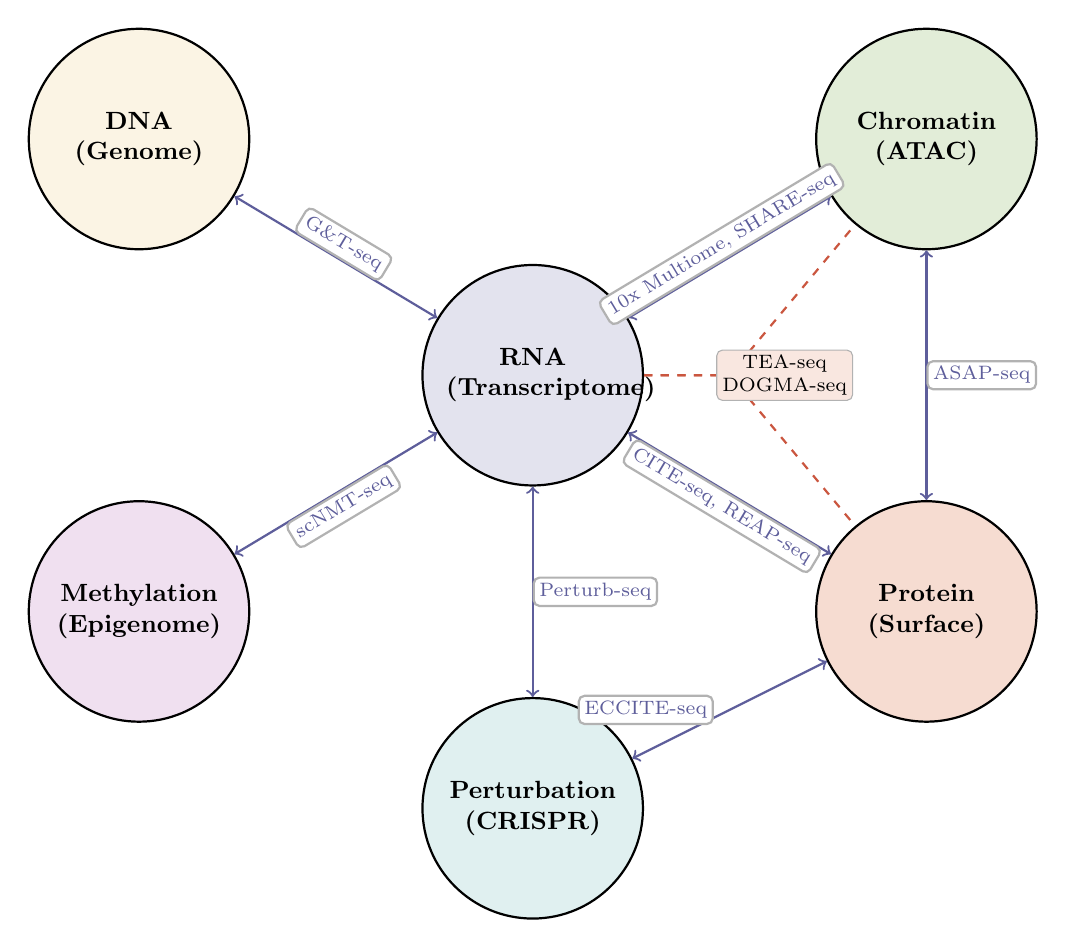
\begin{tikzpicture}[
  modality/.style={
    draw, circle, minimum size=2.8cm, thick,
    font=\small\bfseries, align=center, text width=2.2cm
  },
  method/.style={
    fill=white, draw=gray!60, rounded corners=2pt,
    font=\scriptsize, inner sep=2pt, align=center
  },
  link/.style={thick, MidnightBlue!70, <->},
  triple/.style={thick, BrickRed!70, dashed}
]

% Modality circles
\node[modality, fill=MidnightBlue!12] (rna) at (0,0) {RNA\\(Transcriptome)};
\node[modality, fill=OliveGreen!12] (atac) at (5,3) {Chromatin\\(ATAC)};
\node[modality, fill=BrickRed!12] (protein) at (5,-3) {Protein\\(Surface)};
\node[modality, fill=Goldenrod!12] (dna) at (-5,3) {DNA\\(Genome)};
\node[modality, fill=violet!12] (methyl) at (-5,-3) {Methylation\\(Epigenome)};
\node[modality, fill=teal!12] (perturb) at (0,-5.5) {Perturbation\\(CRISPR)};

% RNA + ATAC links
\draw[link] (rna) -- (atac) node[method, midway, above, sloped] {10x Multiome, SHARE-seq};

% RNA + Protein links
\draw[link] (rna) -- (protein) node[method, midway, below, sloped] {CITE-seq, REAP-seq};

% RNA + DNA links
\draw[link] (rna) -- (dna) node[method, midway, above, sloped] {G\&T-seq};

% RNA + Methylation links
\draw[link] (rna) -- (methyl) node[method, midway, below, sloped] {scNMT-seq};

% ATAC + Protein links
\draw[link] (atac) -- (protein) node[method, midway, right] {ASAP-seq};

% RNA + Perturbation links
\draw[link] (rna) -- (perturb) node[method, midway, right] {Perturb-seq};

% Triple omics (TEA-seq / DOGMA-seq)
\draw[triple] (rna) -- (2.5,0) -- (atac);
\draw[triple] (rna) -- (2.5,0) -- (protein);
\node[method, fill=BrickRed!8] at (3.2,0) {TEA-seq\\DOGMA-seq};

% Protein + Perturbation
\draw[link] (protein) -- (perturb) node[method, midway, left, xshift=-2mm] {ECCITE-seq};

\end{tikzpicture}
\caption[The single-cell multiomics landscape.]{Overview of single-cell multiomics technologies and the molecular modalities they connect. Solid blue arrows indicate dual-modality assays; dashed red lines indicate triple-omics assays. Each technology simultaneously measures the connected modalities from the same individual cell.}
\label{fig:multiomics:landscape}
\end{figure}


\section{Summary}
\label{sec:multiomics:summary}

This chapter has surveyed the rapidly expanding field of single-cell and spatial multiomics. Key takeaways include:

\begin{itemize}[itemsep=3pt]
  \item \textbf{Joint RNA + chromatin:} Technologies such as 10x Multiome and SHARE-seq enable direct linking of regulatory elements to target genes by measuring chromatin accessibility and gene expression in the same cell.
  \item \textbf{Joint RNA + protein:} CITE-seq and related methods provide protein-level cell-type markers alongside whole-transcriptome profiling, bridging the gap between flow cytometry and scRNA-seq.
  \item \textbf{Triple-omics:} TEA-seq and DOGMA-seq achieve simultaneous measurement of RNA, chromatin, and protein, providing the most comprehensive view of single-cell state currently available.
  \item \textbf{Spatial multiomics:} Technologies including spatial-ATAC, CODEX, and DBiT-seq extend multiomics measurements to intact tissues, preserving spatial context.
  \item \textbf{Lineage tracing:} CRISPR barcoding and natural lineage markers (mitochondrial mutations) enable reconstruction of cell lineage trees alongside molecular state.
  \item \textbf{Perturbation screens:} Perturb-seq and CROP-seq map gene function at genome scale by combining CRISPR perturbations with scRNA-seq readout.
  \item \textbf{Computational integration:} The distinction between vertical (same cells), horizontal (same modality), and diagonal (different cells, different modalities) integration is fundamental to choosing appropriate analytical methods.
\end{itemize}

As multiomics technologies continue to mature, their decreasing cost and increasing throughput will make multi-modal profiling the default rather than the exception in single-cell biology, providing an ever more complete picture of cellular identity and function.
